%%%%%%%%%%%%%%%%%%%%%%%%%%%%%%%%%%%%%%%%%%%%%%%%%%%%%%%%%%%%%%%%%%%%%%%%%%%%%%%%%%
\begin{frame}[fragile]\frametitle{}
\begin{center}
{\Large Markov Decision Process}
\end{center}
\end{frame}

%%%%%%%%%%%%%%%%%%%%%%%%%%%%%%%%%%%%%%%%%%%%%%%%%%%%%%%%%%%%%%%%%%%%%%%%%%%%%%%%%%
\begin{frame}[fragile]\frametitle{Definition}

\begin{itemize}
\item State depends only on previous state and action is called as Markov Decision Process.
\item Although in practice, this may not hold true, but thats a simple abstraction that helps formulate Reinforcement Learning algorithm.
\end{itemize}

\end{frame}

%%%%%%%%%%%%%%%%%%%%%%%%%%%%%%%%%%%%%%%%%%%%%%%%%%%%%%%%%%%%%%%%%%%%%%%%%%%%%%%%%%
\begin{frame}[fragile]\frametitle{Fun Example}



\begin{center}
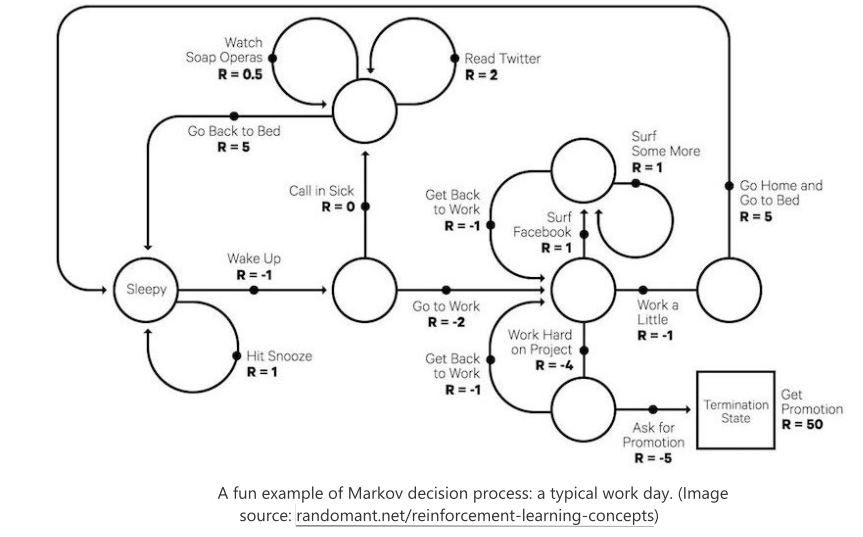
\includegraphics[width=\linewidth,keepaspectratio]{rl99}
\end{center}


{\tiny (Ref: A (Long) Peek into Reinforcement Learning - Lilian Weng)}


\end{frame}

%%%%%%%%%%%%%%%%%%%%%%%%%%%%%%%%%%%%%%%%%%%%%%%%%%%%%%%%%%%%%%%%%%%%%%%%%%%%%%%%%%
\begin{frame}[fragile]\frametitle{Background}

\begin{itemize}
\item Action causes state transitions. Which state it will transition to is probabilistic. $p(s',r|a,s) \neq 1$,meaning,  probability of ending up in a state $s'$, receiving reward $r$, given that you are in state $s$ and have taken action $a$ is not $1$. 
\item $\sum_{s',r} p (s',r|a,s) = 1 $ means $p$ is a probability distribution whose sum of probabilities of all possible states $s'$ and rewards $r$ from a given pair of $(s,a)$ is $1$
\item These probabilities are crucial, they govern how state transitions happen, rewards are calculated, other quantities like Expected Reward.
\item $r(s,a) = E[R_t|S_{t-1}=s,A_{t-1}=a] = \sum_{r \in R} r \times \sum_{s' \in S}  p(s',r|s,a)$, means Expected reward at state $s$ and doing action $a$ is given as sum over all rewards  multiplied by sum over states of all probabilities adding up in those states.
\item Expected returns $G_t$ are sum of all future rewards $R_{t+1} \ldots R_T$ discounted by factor gamma $\gamma$. This, $G_t = R_{t+1} + \gamma R_{t+2} + \gamma^2R_{t+3} + \ldots = \sum_{k=0}^{\infty} \gamma^kR_{t+k+1}$. This summation is possible because Markov forces the dependence only on the previous state (proof?)
\end{itemize}

{\tiny (Ref: Modern Reinforcement Learning: Deep Q Learning in PyTorch - Phil Tabor)}

\end{frame}

%%%%%%%%%%%%%%%%%%%%%%%%%%%%%%%%%%%%%%%%%%%%%%%%%%%%%%%%%%%%%%%%%%%%%%%%%%%%%%%%%%
\begin{frame}[fragile]\frametitle{Background}

\begin{itemize}
\item How do we know what future returns would be? meaning, future discounted rewards would be? for that, we will need what future actions would be? how to know that?
\item Here comes Policy, which predicts actions based on current state, probabilistically. $\pi(s,a)$ is probability of selecting $a$ being at $s$.
\item So at any point in time, ie in any state, for any action, we would be in position to calculate expected returns for all possible paths emanating from there.
\item Thus the position, ie, the state (and state+action) has certain value associated with it.
\end{itemize}

{\tiny (Ref: Modern Reinforcement Learning: Deep Q Learning in PyTorch - Phil Tabor)}

\end{frame}

%%%%%%%%%%%%%%%%%%%%%%%%%%%%%%%%%%%%%%%%%%%%%%%%%%%%%%%%%%%%%%%%%%%%%%%%%%%%%%%%%%
\begin{frame}[fragile]\frametitle{Value Functions}


\begin{itemize}
\item Evaluation of a position on board, ie state.
\item Two types:
	\begin{itemize}
	\item State Value Function: Expected returns for state $s$ with policy $\pi$ is $v_{\pi}(s) = E_{\pi}[G_t|S_t=s]$
	\item Action Value Function: Expected returns for taking action $a$ atstate $s$ with policy $\pi$ is $q_{\pi}(s,a) = E_{\pi}[G_t|S_t=s, A_t=a]$
	\end{itemize}

\end{itemize}



{\tiny (Ref: Solving Tic-Tac-Toe with Reinforcement Learning - Govind G Nair)}

\end{frame}

%%%%%%%%%%%%%%%%%%%%%%%%%%%%%%%%%%%%%%%%%%%%%%%%%%%%%%%%%%%%%%%%%%%%%%%%%%%%%%%%%%
\begin{frame}[fragile]\frametitle{Value Functions}

\begin{itemize}
\item Goodness or value of state (or state-action) is, better $G_t$ from it, larger the value.
\item Value of a state $s$ according to policy $\pi$ is given as $v_{\pi}(s) = E_{\pi}[G_t|S_t=s]=E_{\pi}[\sum_{k=0}^{\infty}\gamma^kR_{t+k+1}|S_t=s] \forall s \in S$
\item Value of $s-a$ pair is decided by function $q_{\pi}$ and is very similar to above with just action component added to it. $q_{\pi}(s,a) = E_{\pi}[G_t|S_t=s, A_t=a]=E_{\pi}[\sum_{k=0}^{\infty}\gamma^kR_{t+k+1}|S_t=s, A_t=a] \forall s \in S$
\item Q in the Q-Learning is the above $q$!! It denotes Quality.
\item How do you get the Expectation value, the $E$ in the equation above without probabilities (Note: Expected = outcome x probabilities = Sum of Rewards x Sum of Probabilities of State-Actions). The 2nd term is related to Policy.
\end{itemize}

{\tiny (Ref: Modern Reinforcement Learning: Deep Q Learning in PyTorch - Phil Tabor)}

\end{frame}

%%%%%%%%%%%%%%%%%%%%%%%%%%%%%%%%%%%%%%%%%%%%%%%%%%%%%%%%%%%%%%%%%%%%%%%%%%%%%%%%%%
\begin{frame}[fragile]\frametitle{Bellman Equation}

\begin{itemize}
\item Plug formula for $G_t$ in value function $v_{\pi}$. So $v_{\pi}(s) = E_{\pi}[G_t|S_t=s]$, with $G_t = R_{t+1}+ \gamma G_{t+1}$ becomes $v_{\pi}(s) = E_{\pi}[R_{t+1}+ \gamma G_{t+1}|S_t=s]$. Note there is no $\gamma^k$ term like it was there in original $v_{\pi}$ formula.
\item Expanding for $R_{t+1}$ for certain policy $\pi$ is $\sum_a \pi(a,s) \sum_s' \sum_r p(s',r|s,a) [r + \gamma E_{\pi} [G_{t+1}|S_{t+1}=s']]$, the last term is same as value function at time step $t+1$
\item $v_{\pi}(s) = \sum_a \pi(a,s) \sum_s' \sum_r p(s',r|s,a) [r + \gamma v_{\pi}(s')]$ meaning, value function for policy $\pi$ for a state $s$ is = sum over all possible actions $a$ at state $s$ for the given policy $\pi$ multiplied by sum over all possible future states $s'$ and rewards $r$, the probability distribution of states $s'$ and rewards $r$ given current state $s$ and action $a$ times reward $r$ plus $\gamma$ times value of the next state $s'$
\item This is Bellman Equation and solving is core of the Reinforcement Learning formulation. Is a relation of value of current state with respect to value of future states. A forward recursion.
\end{itemize}

{\tiny (Ref: Modern Reinforcement Learning: Deep Q Learning in PyTorch - Phil Tabor)}

\end{frame}


%%%%%%%%%%%%%%%%%%%%%%%%%%%%%%%%%%%%%%%%%%%%%%%%%%%%%%%%%%%%%%%%%%%%%%%%%%%%%%%%%%
\begin{frame}[fragile]\frametitle{Bellman Equations}


\begin{columns}
\begin{column}{0.5\textwidth}
\begin{itemize}
\item The value of a state $s$  is obtained by considering all possible paths to all possible successor states , and weighting the rewards obtained and value of these successor states by the probabilities of taking each path.
\item $V_{\pi}(B) = 0.5V_{\pi}(D) + 0.5V_{\pi}(E) = 0.5 x 4+ 0.5 x 3 = 3.5$
\end{itemize}

\end{column}
\begin{column}{0.5\textwidth}  %%<--- here
\begin{center}
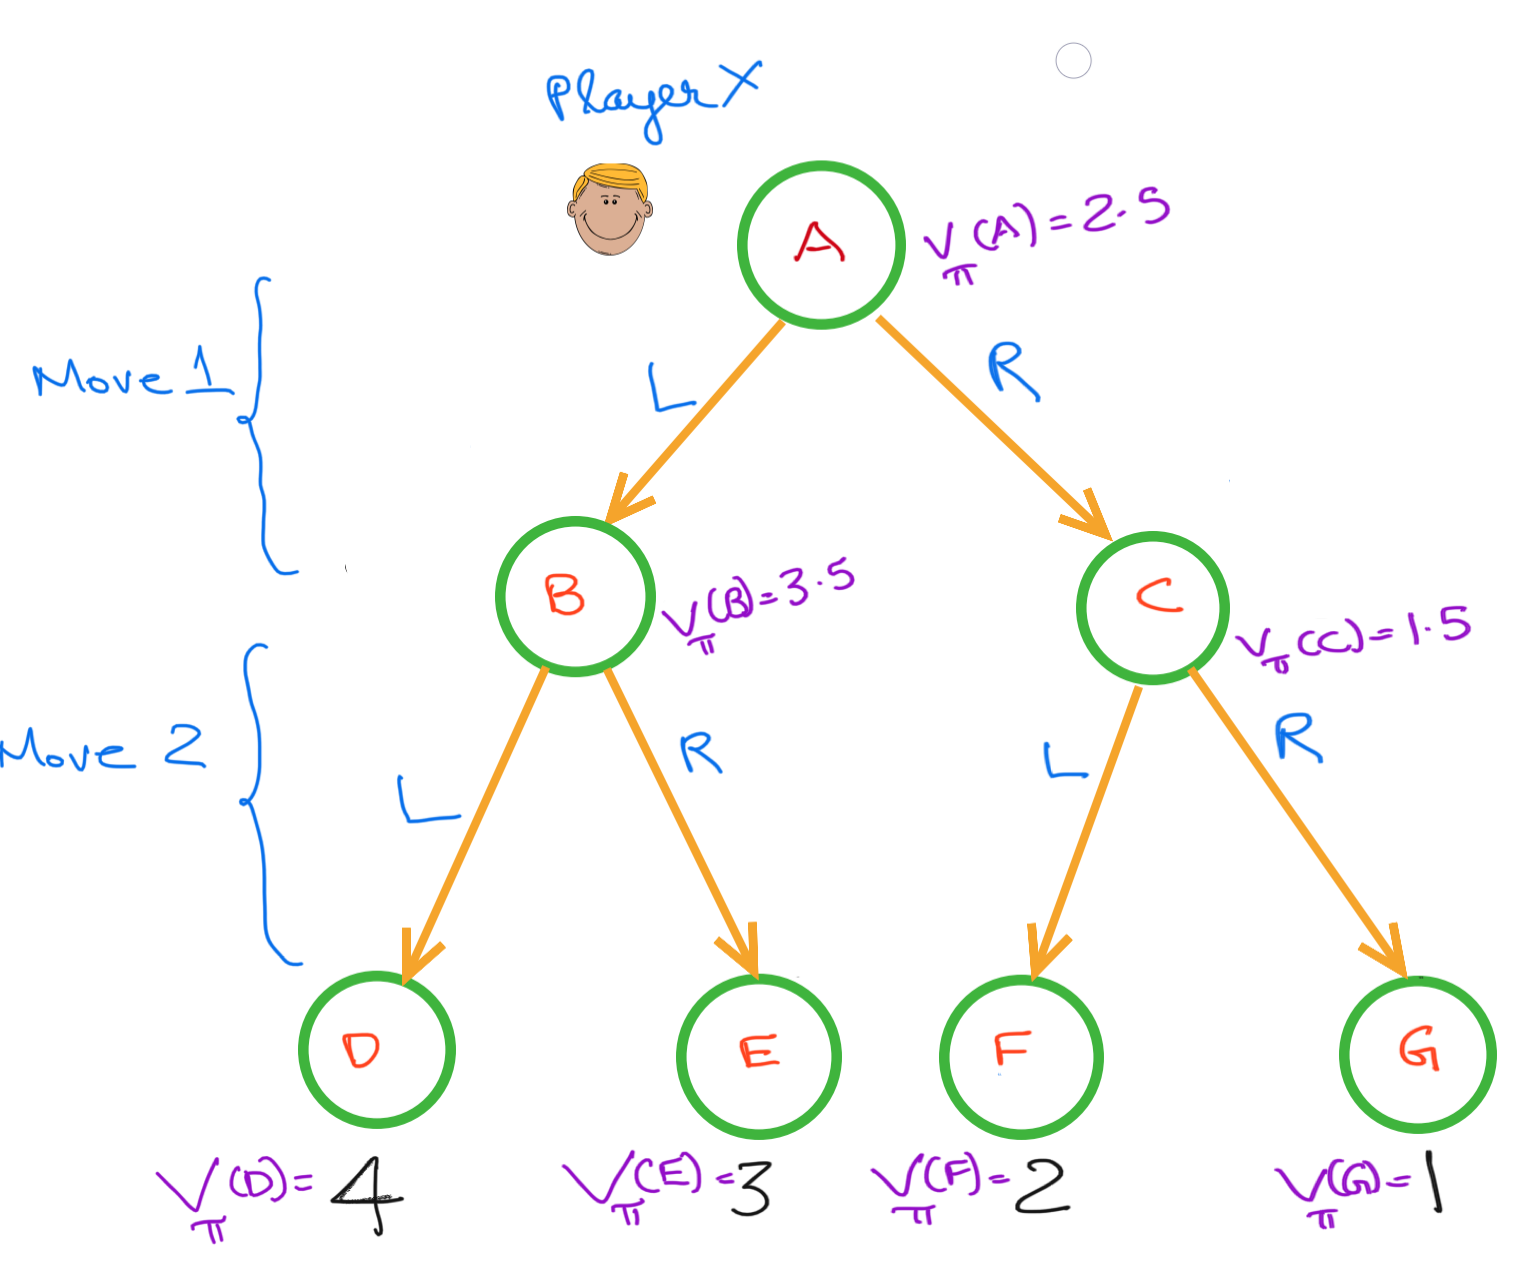
\includegraphics[width=0.8\linewidth,keepaspectratio]{rl73}
\end{center}
\end{column}
\end{columns}

{\tiny (Ref: Solving Tic-Tac-Toe with Reinforcement Learning - Govind G Nair)}

\end{frame}


%%%%%%%%%%%%%%%%%%%%%%%%%%%%%%%%%%%%%%%%%%%%%%%%%%%%%%%%%%%%%%%%%%%%%%%%%%%%%%%%%%
\begin{frame}[fragile]\frametitle{Bellman Equations}



\begin{itemize}
\item Once the value of the successive states are known, the agent can pick the action that leads to the optimal state. In this example, the agent wants to move to state B, and takes action “L” to move to that state. A limitation of the state value function is that once you have determined the optimal state, you have to then identify the action that leads to that state.
\item The action value function does not have this limitation, it directly gives the value of each action at a given state making it easy to pick the optimal actions.
\item The action-value function at states B, C and A are given by
\end{itemize}


\begin{align*}
Q(\mathcal{S}=B,\mathcal{A}=L) &= 4\\
Q(\mathcal{S}=B,\mathcal{A}=R) &= 3\\
Q(\mathcal{S}=C,\mathcal{A}=L) &= 2\\
Q(\mathcal{S}=C,\mathcal{A}=R) &= 1\\
Q(\mathcal{S}=A,\mathcal{A}=L) &= 3.5\\
Q(\mathcal{S}=A,\mathcal{A}=R) &= 1.5
\end{align*}


{\tiny (Ref: Solving Tic-Tac-Toe with Reinforcement Learning - Govind G Nair)}

\end{frame}

%%%%%%%%%%%%%%%%%%%%%%%%%%%%%%%%%%%%%%%%%%%%%%%%%%%%%%%%%%%%%%%%%%%%%%%%%%%%%%%%%%
\begin{frame}[fragile]\frametitle{Advantage  functions}

\begin{itemize}
\item Sometimes in RL, we don’t need to describe how good an action is in an absolute sense, but only how much better it is than others on average. That is to say, we want to know the relative advantage of that action. 
\item We make this concept precise with the advantage function.
\item The advantage function $A^{\pi}(s,a)$ corresponding to a policy $\pi$ describes how much better it is to take a specific action a in state $s$, over randomly selecting an action according to $\pi(\cdot|s)$, assuming you act according to $\pi$ forever after. Mathematically, the advantage function is defined by $A^{\pi}(s,a) = Q^{\pi}(s,a) - V^{\pi}(s)$.
\end{itemize}

{\tiny (Ref: Spinning Up - Open AI)}
\end{frame}



%%%%%%%%%%%%%%%%%%%%%%%%%%%%%%%%%%%%%%%%%%%%%%%%%%%%%%%%%%%%%%%%%%%%%%%%%%%%%%%%%%
\begin{frame}[fragile]\frametitle{Common Approaches}

Major approaches and classic algorithms for solving RL
problems. 

\begin{itemize}
\item Dynamic Programming: When the model is fully known, following Bellman equations, we can use Dynamic Programming (DP)
to iteratively evaluate value functions and improve policy.
\item Monte-Carlo Methods:  uses a simple idea: It learns
from episodes of raw experience without modeling the environmental dynamics and computes the
observed mean return as an approximation of the expected return.
\item Temporal-Difference Learning: Similar to Monte-Carlo methods, Temporal-Difference (TD) Learning is model-free and learns from
episodes of experience. However, TD learning can learn from incomplete episodes and hence we
don’t need to track the episode up to termination.

\end{itemize}


{\tiny (Ref: A (Long) Peek into Reinforcement Learning - Lilian Weng)}


\end{frame}

%%%%%%%%%%%%%%%%%%%%%%%%%%%%%%%%%%%%%%%%%%%%%%%%%%%%%%%%%%%%%%%%%%%%%%%%%%%%%%%%%%
\begin{frame}[fragile]\frametitle{TD Control}

\begin{itemize}
\item Bootstrapping: TD learning methods update targets with regard to existing estimates rather than exclusively relying
on actual rewards and complete returns as in MC methods
\item Value Estimation: The key idea in TD learning is to update the value function $V(s_t)$ towards an estimated return
\item SARSA: On-Policy TD control:  updating Q-value by following a sequence of $\ldots , S_t,A_t,R_{t+1}, S_{t+1},\ldots$
\item Q-Learning: Off-policy TD control: The key difference from SARSA is that Q-learning does not follow the current policy to pick the
second action $A_{t+1}$, but it estimates $Q*$ out of the best $Q$ values, but which action (denoted as $a*$) leads to this maximal $Q$ does not matter  and the next step $Q$ learning many not follow $a*$.
\item Deep Q-network: For larges state space, use Machine/Deep Learning to approximate $Q$ values.
\end{itemize}




{\tiny (Ref: A (Long) Peek into Reinforcement Learning - Lilian Weng)}


\end{frame}


%%%%%%%%%%%%%%%%%%%%%%%%%%%%%%%%%%%%%%%%%%%%%%%%%%%%%%%%%%%%%%%%%%%%%%%%%%%%%%%%%%
\begin{frame}[fragile]\frametitle{Optimal Policy}

For any MDP:

\begin{itemize}
\item There exists an optimal policy$\pi$, that is better than or equal to all other policies, $\pi_* \geq \pi, \forall \pi$
\item All optimal policies achieve the optimal value function $v_{\pi_*}(s) = v_*(s)$
\item All optimal policies achieve optimal action-value function,  $q_{\pi_*}(s,a) = q_*(s,a)$
\item An optimal policy can be found by maximizing over the optimal value function $\pi_*(s) = arg_a max q_*(s,a)$
\item  $q_*(s,a)$ is given by the ``Bellman optimality equations''
\item All RL algorithms solve for the Bellman Equations exactly or approximately. 
\end{itemize}



{\tiny (Ref: Solving Tic-Tac-Toe with Reinforcement Learning - Govind G Nair)}

\end{frame}

%%%%%%%%%%%%%%%%%%%%%%%%%%%%%%%%%%%%%%%%%%%%%%%%%%%%%%%%%%%%%%%%%%%%%%%%%%%%%%%%%%
\begin{frame}[fragile]\frametitle{The Optimal Q-Function and the Optimal Action}

\begin{itemize}
\item There is an important connection between the optimal action-value function $Q^*(s,a)$ and the action selected by the optimal policy. 
\item By definition, $Q^*(s,a)$ gives the expected return for starting in state $s$, taking (arbitrary) action $a$, and then acting according to the optimal policy forever after.
\item The optimal policy in s will select whichever action maximizes the expected return from starting in $s$. As a result, if we have $Q^*$, we can directly obtain the optimal action, $a^*(s)$, via $a^*(s) = \arg \max_a Q^* (s,a)$.
\item Note: there may be multiple actions which maximize $Q^*(s,a)$, in which case, all of them are optimal, and the optimal policy may randomly select any of them. But there is always an optimal policy which deterministically selects an action.
\end{itemize}

{\tiny (Ref: Spinning Up - Open AI)}
\end{frame}


%%%%%%%%%%%%%%%%%%%%%%%%%%%%%%%%%%%%%%%%%%%%%%%%%%%%%%%%%%%%%%%%%%%%%%%%%%%%%%%%%%
\begin{frame}[fragile]\frametitle{Ranking}


\begin{itemize}
\item Given Bellman Equation, can be evaluate different policies?
\item Yes, in fact, the whole point of $v$ and $q$ is to rank policies.
\item So if one policy has better values for all states than the values for any other policy, then the first one is better.
\item Value of a state is max of value from state-action pairs. $v_*(s) = max q_{\pi_*}(s,a)$
\item By substitution, $v_*(s) = max E_{\pi}[G_t|S_t=s, A_t=a] = max E_{\pi}[R_{t+1}+ \gamma G_{t+1}|S_t=s, A_t=a] = max \sum_{s',r} p (s',r|s,a)[r + \gamma v_*(s')]$. Similarly $q*(s,a) = \sum_{s',r} p (s',r|s,a)[r + \gamma max q_*(s',a')]$
\item This is Bellman Optimality Equation.
\end{itemize}

{\tiny (Ref: Modern Reinforcement Learning: Deep Q Learning in PyTorch - Phil Tabor)}

\end{frame}

%%%%%%%%%%%%%%%%%%%%%%%%%%%%%%%%%%%%%%%%%%%%%%%%%%%%%%%%%%%%%%%%%%%%%%%%%%%%%%%%%%
\begin{frame}[fragile]\frametitle{Probability}

$v_{\pi}(s) = \sum_a \pi(a,s) \sum_s' \sum_r p(s',r|s,a) [r + \gamma v_{\pi}(s')]$

\begin{itemize}
\item Probability distribution term $p$ in the Bellman equation is unknown.
\item Suppose we know the probability distribution, then we the policy also and rewards, thus we have everything to calculate Bellman Equation. Thats like Exploitation.
\item For Terminal ie last state, the returns $G_T = 0$ so $v_{\pi}(s_T) = E_{\pi}[G_T|S=s_T] =E[0] 0$. Using that on right hand side, calculate one step back ie time step $T-1$, and so on.
\item Known Probability Distribution means whole model is known. Thats Dynamic Programming.
\item For Unknown Probability Function, other methods like Q-Learning are used. Thats Model-Free way. Here $p$ is decided by trial and error with playing in the Environment. Thats more of Exploration.
\end{itemize}

{\tiny (Ref: Modern Reinforcement Learning: Deep Q Learning in PyTorch - Phil Tabor)}

\end{frame}

%%%%%%%%%%%%%%%%%%%%%%%%%%%%%%%%%%%%%%%%%%%%%%%%%%%%%%%%%%%%%%%%%%%%%%%%%%%%%%%%%%
\begin{frame}[fragile]\frametitle{Temporal Difference Learning}

$v_{\pi}(s) = \sum_a \pi(a,s) \sum_s' \sum_r p(s',r|s,a) [r + \gamma v_{\pi}(s')]$

\begin{itemize}
\item Value function is the Expected return for given state for given action according to given policy.
\item Initially all values for all states is say 0. Need to update each using the value function formlua.
\item Randomly select any state, calculate and update $v$, do this many times so that the $v$ converges to some single value in each state. Imagine tabular state action method for small number of states like Frozen Lake problem.
\item New Estimate = Old estimate + step size x (Target - Old Estimate)
\item Here Target is the required Reward at that time-step given. Thats Q Learning. In Monte Carlo, estimates are updated at the end of the episode.
\item $V(s_t) = V(s_t) + \alpha ( R_{t+1} + \gamma V(s_{t+1}) - V(s_t))$, Similarly for Q, ie state-action value function, $Q(s_t,a_t) = Q(s_t,a_t) + \alpha ( R_{t+1} + \gamma max Q(s_{t+1},a_{max}) - Q(s_t,a_t))$
\item Thus Q Learning is Online Learning  and also suitable for continuous tasks.
\item If policy for prediction of action and estimating q value, are different then thats OFF Policy, if same thats ON POLICY (ToDO: need to confirm this!!)
\end{itemize}

{\tiny (Ref: Modern Reinforcement Learning: Deep Q Learning in PyTorch - Phil Tabor)}

\end{frame}

%%%%%%%%%%%%%%%%%%%%%%%%%%%%%%%%%%%%%%%%%%%%%%%%%%%%%%%%%%%%%%%%%%%%%%%%%%%%%%%%%%
\begin{frame}[fragile]\frametitle{Policy Gradient}

\begin{itemize}
\item All the methods we have introduced above aim to learn the state/action value function and then to
select actions accordingly. 
\item Policy Gradient methods instead learn the policy directly with a parameterized function respect to $\theta,\pi(a|s;\theta)$
\item Let’s define the reward function (opposite of loss
function) as the expected return and train the algorithm with the goal to maximize the reward function.
\item Using gradient ascent we can find the best $\theta$ that produces the highest return. It is natural to expect
policy-based methods are more useful in continuous space, because there is an infinite number of
actions and/or states to estimate the values for in continuous space and hence value-based
approaches are computationally much more expensive.
\end{itemize}

{\tiny (Ref: A (Long) Peek into Reinforcement Learning - Lilian Weng)}


\end{frame}

%%%%%%%%%%%%%%%%%%%%%%%%%%%%%%%%%%%%%%%%%%%%%%%%%%%%%%%%%%%%%%%%%%%%%%%%%%%%%%%%%%
\begin{frame}[fragile]\frametitle{What are Policy-Gradient Methods?}

\begin{itemize}
\item Policy-Gradient is a subclass of Policy-Based Methods, a category of algorithms that aims to optimize the policy directly without using a value function using different techniques. 
\item The difference with Policy-Based Methods is that Policy-Gradient methods are a series of algorithms that aim to optimize the policy directly by estimating the weights of the optimal policy using Gradient Ascent.
\end{itemize}

{\tiny (Ref: Chapter 5 of the Deep Reinforcement Learning Class with Hugging Face)}

\end{frame}

%%%%%%%%%%%%%%%%%%%%%%%%%%%%%%%%%%%%%%%%%%%%%%%%%%%%%%%%%%%%%%%%%%%%%%%%%%%%%%%%%%
\begin{frame}[fragile]\frametitle{Overview }

Our goal with Policy-Gradients is to control the probability distribution of actions by tuning the policy such that good actions (that maximize the return) are sampled more frequently in the future.

A simple example:
 
\begin{itemize}
\item We collect an episode by letting our policy interact with its environment.
\item We then look at the sum of rewards of the episode (expected return). If this sum is positive, we consider that the actions taken during the episodes were good: Therefore, we want to increase the P(a|s) (probability of taking that action at that state) for each state-action pair.
\item But value based Deep Q-Learning is excellent! then, Why use policy gradient methods?
\end{itemize}

{\tiny (Ref: Chapter 5 of the Deep Reinforcement Learning Class with Hugging Face)}

\end{frame}

%%%%%%%%%%%%%%%%%%%%%%%%%%%%%%%%%%%%%%%%%%%%%%%%%%%%%%%%%%%%%%%%%%%%%%%%%%%%%%%%%%
\begin{frame}[fragile]\frametitle{Advantages  }

\begin{itemize}
\item The simplicity of the integration: we can estimate the policy directly without storing additional data (action values).
\item Policy gradient methods can learn a stochastic policy while value functions can't.
\end{itemize}

This has two consequences:

\begin{itemize}
\item We don't need to implement an exploration/exploitation trade-off by hand. Since we output a probability distribution over actions, the agent explores the state space without always taking the same trajectory.
\item We also get rid of the problem of perceptual aliasing. Perceptual aliasing is when two states seem (or are) the same but need different actions.
\end{itemize}
{\tiny (Ref: Chapter 5 of the Deep Reinforcement Learning Class with Hugging Face)}

\end{frame}

%%%%%%%%%%%%%%%%%%%%%%%%%%%%%%%%%%%%%%%%%%%%%%%%%%%%%%%%%%%%%%%%%%%%%%%%%%%%%%%%%%
\begin{frame}[fragile]\frametitle{Example  }

\begin{itemize}
\item We have an intelligent vacuum cleaner whose goal is to suck the dust and avoid killing the hamsters.
\item Our vacuum cleaner can only perceive where the walls are.
\item The problem is that the two red cases are aliased states because the agent perceives an upper and lower wall for each.
\end{itemize}

\begin{center}
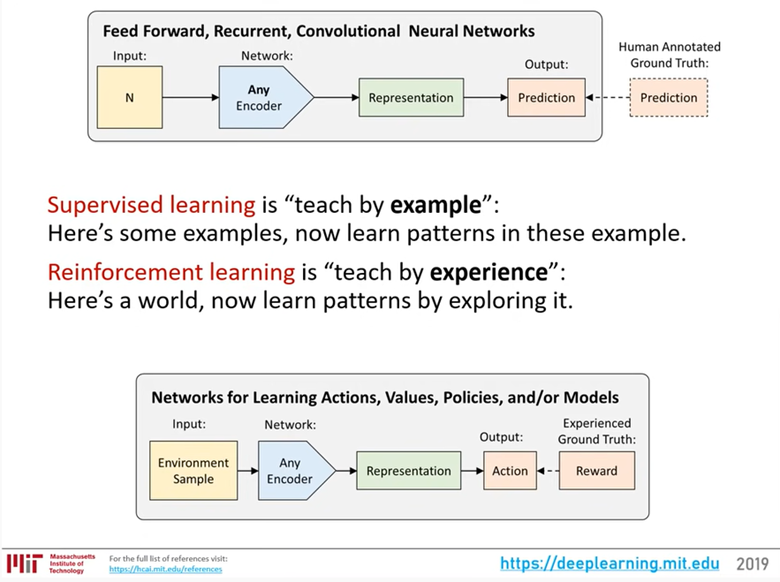
\includegraphics[width=0.6\linewidth,keepaspectratio]{rl25}

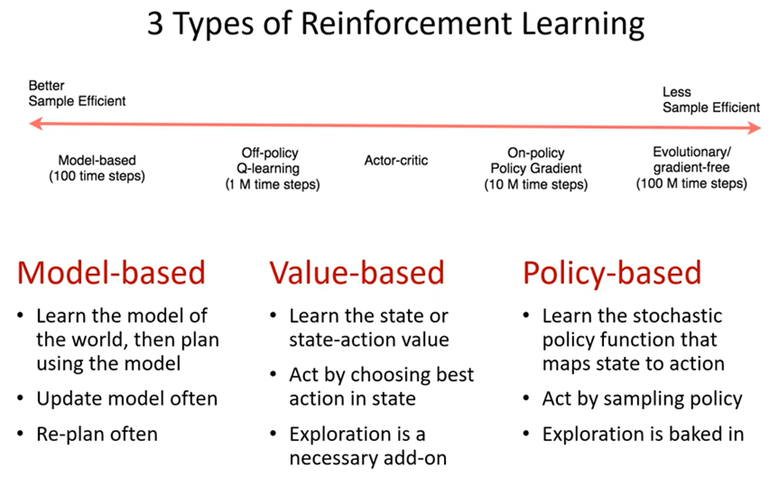
\includegraphics[width=0.6\linewidth,keepaspectratio]{rl26}

\end{center}

{\tiny (Ref: Chapter 5 of the Deep Reinforcement Learning Class with Hugging Face)}

\end{frame}


%%%%%%%%%%%%%%%%%%%%%%%%%%%%%%%%%%%%%%%%%%%%%%%%%%%%%%%%%%%%%%%%%%%%%%%%%%%%%%%%%%
\begin{frame}[fragile]\frametitle{Example  }

\begin{itemize}
\item Under a deterministic policy, the policy will either move right when in a red state or move left. Either case will cause our agent to get stuck and never suck the dust.

\item Under a value-based RL algorithm, we learn a quasi-deterministic policy ("greedy epsilon strategy"). Consequently, our agent can spend a lot of time before finding the dust.

\item On the other hand, an optimal stochastic policy will randomly move left or right in grey states. Consequently, it will not be stuck and will reach the goal state with a high probability.

\item Policy gradients are more effective in high-dimensional action spaces and continuous actions spaces
\end{itemize}

\begin{center}
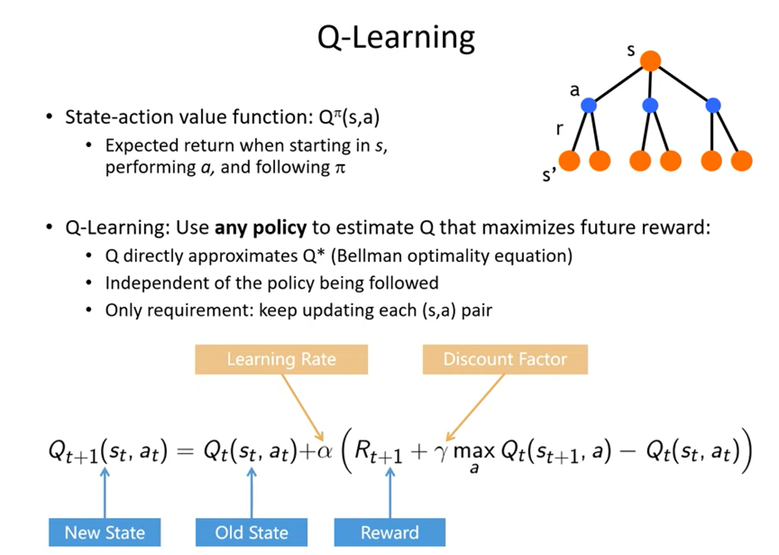
\includegraphics[width=0.6\linewidth,keepaspectratio]{rl27}
\end{center}

{\tiny (Ref: Chapter 5 of the Deep Reinforcement Learning Class with Hugging Face)}

\end{frame}

%%%%%%%%%%%%%%%%%%%%%%%%%%%%%%%%%%%%%%%%%%%%%%%%%%%%%%%%%%%%%%%%%%%%%%%%%%%%%%%%%%
\begin{frame}[fragile]\frametitle{Example  }

\begin{itemize}
\item Indeed, the problem with Deep Q-learning is that their predictions assign a score (maximum expected future reward) for each possible action, at each time step, given the current state.

\item But what if we have an infinite possibility of actions?

\item For instance, with a self-driving car, at each state, you can have a (near) infinite choice of actions (turning the wheel at 15, 17.2, 19,4, honking, etc.). We'll need to output a Q-value for each possible action! And taking the max action of a continuous output is an optimization problem itself!

\item Instead, with a policy gradient, we output a probability distribution over actions.
\end{itemize}

{\tiny (Ref: Chapter 5 of the Deep Reinforcement Learning Class with Hugging Face)}

\end{frame}

%%%%%%%%%%%%%%%%%%%%%%%%%%%%%%%%%%%%%%%%%%%%%%%%%%%%%%%%%%%%%%%%%%%%%%%%%%%%%%%%%%
\begin{frame}[fragile]\frametitle{Disadvantages   }

\begin{itemize}
\item Policy gradients converge a lot of time on a local maximum instead of a global optimum.
\item Policy gradient goes faster, step by step: it can take longer to train (inefficient).
\item Policy gradient can have high variance (solution baseline).
\end{itemize}

{\tiny (Ref: Chapter 5 of the Deep Reinforcement Learning Class with Hugging Face)}

\end{frame}


%%%%%%%%%%%%%%%%%%%%%%%%%%%%%%%%%%%%%%%%%%%%%%%%%%%%%%%%%%%%%%%%%%%%%%%%%%%%%%%%%%
\begin{frame}[fragile]\frametitle{Reinforce (Monte Carlo Policy Gradient)}

\begin{itemize}
\item Reinforce, also called Monte-Carlo Policy Gradient, uses an estimated return from an entire episode to update the policy parameter $\theta$.
\item We have our policy  $\pi$ which has a parameter $\theta$. This $\pi$, given a state, outputs a probability distribution of actions.
\item $\pi_\theta(a|s) = p[a|s;\theta]$ Where $\pi_\theta(a_t|s_t)$ is the probability of the agent selecting action at from state $s_t$, given our policy.
\item Measure goodness by core/objective function called $J(\theta)$.
\end{itemize}


\begin{center}
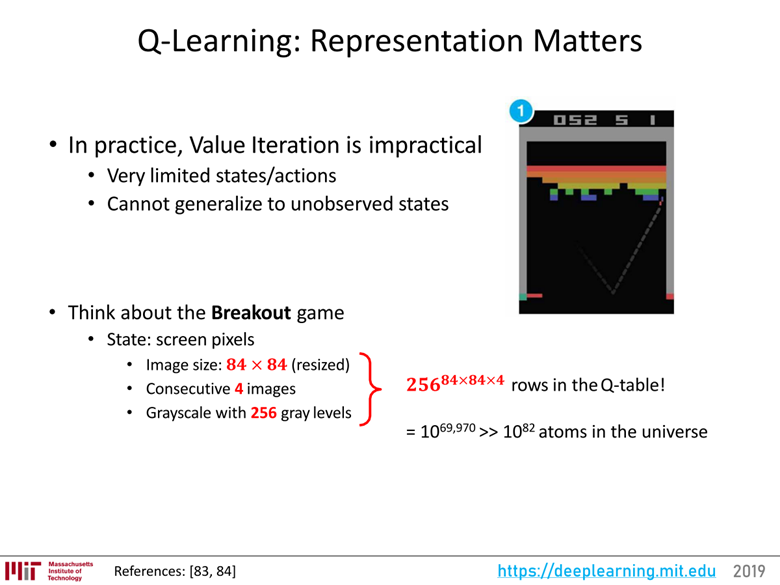
\includegraphics[width=0.6\linewidth,keepaspectratio]{rl28}
\end{center}

{\tiny (Ref: Chapter 5 of the Deep Reinforcement Learning Class with Hugging Face)}

\end{frame}


%%%%%%%%%%%%%%%%%%%%%%%%%%%%%%%%%%%%%%%%%%%%%%%%%%%%%%%%%%%%%%%%%%%%%%%%%%%%%%%%%%
\begin{frame}[fragile]\frametitle{Reinforce (Monte Carlo Policy Gradient)}

\begin{itemize}
\item Remember that policy gradient can be seen as an optimization problem. So we must find the best parameters $\theta$ to maximize the score function, $J(\theta)$.

\item To do that we’re going to use the Policy Gradient Theorem. 
\item The Reinforce algorithm works like this: Loop:
\begin{itemize}
\item Use the policy $\pi_\theta$ to collect an episode $\tau$
\item Use the episode to estimate the gradient $\hat{g} = \nabla_\theta J(\theta)$ 
\item Update the weights of the policy: $\theta \leftarrow \theta + \alpha \hat{g}$
\end{itemize}
\end{itemize}

{\tiny (Ref: Chapter 5 of the Deep Reinforcement Learning Class with Hugging Face)}

\end{frame}



%%%%%%%%%%%%%%%%%%%%%%%%%%%%%%%%%%%%%%%%%%%%%%%%%%%%%%%%%%%%%%%%%%%%%%%%%%%%%%%%%%
\begin{frame}[fragile]\frametitle{Reinforce (Monte Carlo Policy Gradient)}

The interpretation we can make is this one:

\begin{itemize}
\item $\triangledown_\theta \log\pi_\theta(a_t,s_t)$  is the direction of steepest increase of the (log) probability of selecting action at from state  $s_t$. 
\item This tells use how we should change the weights of policy if we want to increase/decrease the log probability of selecting action at at state $s_t$.
\item $R(\tau)$: is the scoring function::
\begin{itemize}
\item If the return is high, it will push up the probabilities of the (state, action) combinations.
\item Else, if the return is low, it will push down the probabilities of the (state, action) combinations.
\end{itemize}
\end{itemize}

{\tiny (Ref: Chapter 5 of the Deep Reinforcement Learning Class with Hugging Face)}

\end{frame}


%%%%%%%%%%%%%%%%%%%%%%%%%%%%%%%%%%%%%%%%%%%%%%%%%%%%%%%%%%%%%%%%%%%%%%%%%%%%%%%%%%
\begin{frame}[fragile]\frametitle{}
\begin{center}
{\Large Example}
\end{center}
\end{frame}



%%%%%%%%%%%%%%%%%%%%%%%%%%%%%%%%%%%%%%%%%%%%%%%%%%%%%%%%%%%%%%%%%%%%%%%%%%%%%%%%%%
\begin{frame}[fragile]\frametitle{Example}

Here is one example. Agent (orange ball) tries to collect reward or gets penalty (both terminal states)

\begin{center}
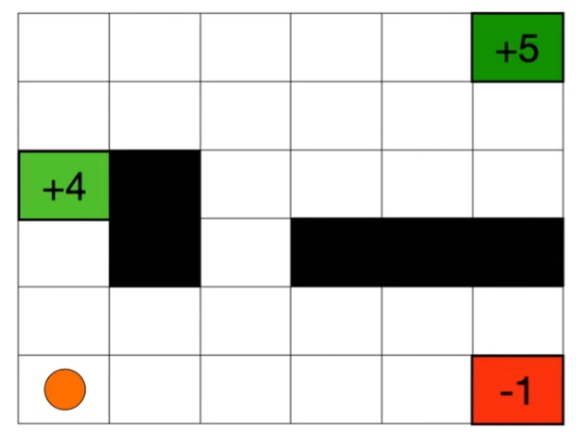
\includegraphics[width=0.6\linewidth,keepaspectratio]{rl34}
\end{center}

{\tiny (Ref: A friendly introduction to deep reinforcement learning, Q-networks and policy gradients)}

\end{frame}

%%%%%%%%%%%%%%%%%%%%%%%%%%%%%%%%%%%%%%%%%%%%%%%%%%%%%%%%%%%%%%%%%%%%%%%%%%%%%%%%%%
\begin{frame}[fragile]\frametitle{Example}

Value of a state is max of its values of neighbors $=>$ Bellman equation

\begin{center}
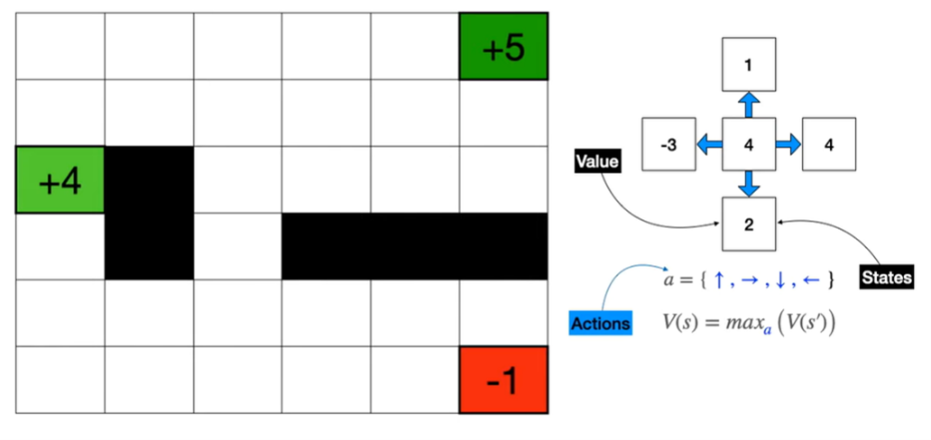
\includegraphics[width=0.8\linewidth,keepaspectratio]{rl35}
\end{center}

{\tiny (Ref: A friendly introduction to deep reinforcement learning, Q-networks and policy gradients)}

\end{frame}

%%%%%%%%%%%%%%%%%%%%%%%%%%%%%%%%%%%%%%%%%%%%%%%%%%%%%%%%%%%%%%%%%%%%%%%%%%%%%%%%%%
\begin{frame}[fragile]\frametitle{Example}

At start, we know value of only the terminal states. Rest is blank. But we can fill them by above mentioned nationhood logic.

\begin{center}
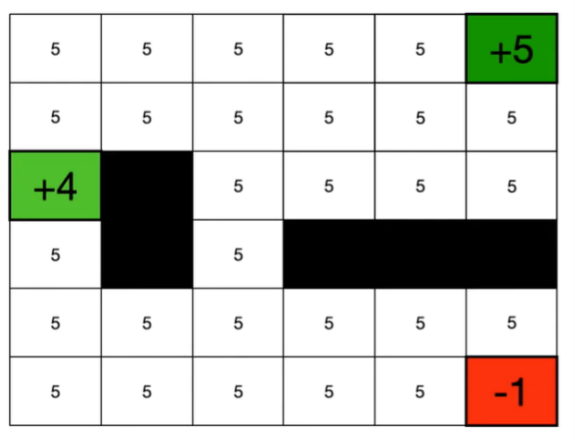
\includegraphics[width=0.6\linewidth,keepaspectratio]{rl36}
\end{center}

{\tiny (Ref: A friendly introduction to deep reinforcement learning, Q-networks and policy gradients)}

\end{frame}

%%%%%%%%%%%%%%%%%%%%%%%%%%%%%%%%%%%%%%%%%%%%%%%%%%%%%%%%%%%%%%%%%%%%%%%%%%%%%%%%%%
\begin{frame}[fragile]\frametitle{Example}

Policy is set of decision to take the agent to best possible path, say, a set of arrows here. So, need to avoid -1 and 4 but try 5. Also avoiding the walls. Still looks inefficient. Try to get faster than go here and there. Use Rewards/Penalties to minimize the steps needed. Assume each steps costs agent 1. So, when Agent moves to ‘4’ state, s/he gets 4-1 = 3. Do this for all neighbors and then take max. From each state, you can go only in the direction (arrow) if the value is higher and not reverse.

\begin{center}
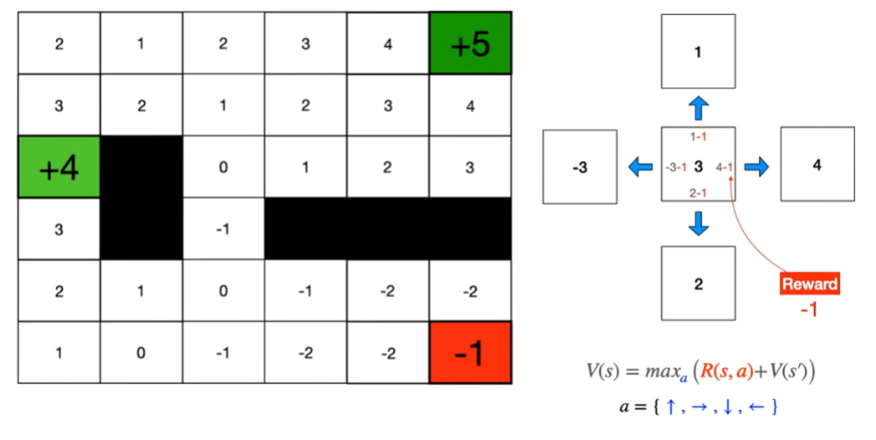
\includegraphics[width=0.6\linewidth,keepaspectratio]{rl37}
\end{center}

{\tiny (Ref: A friendly introduction to deep reinforcement learning, Q-networks and policy gradients)}

\end{frame}

%%%%%%%%%%%%%%%%%%%%%%%%%%%%%%%%%%%%%%%%%%%%%%%%%%%%%%%%%%%%%%%%%%%%%%%%%%%%%%%%%%
\begin{frame}[fragile]\frametitle{Example}

\begin{center}
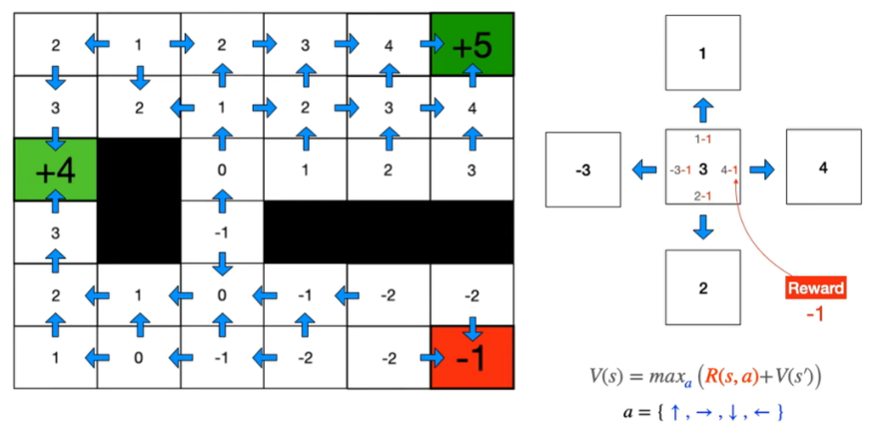
\includegraphics[width=0.8\linewidth,keepaspectratio]{rl38}
\end{center}

{\tiny (Ref: A friendly introduction to deep reinforcement learning, Q-networks and policy gradients)}

\end{frame}

%%%%%%%%%%%%%%%%%%%%%%%%%%%%%%%%%%%%%%%%%%%%%%%%%%%%%%%%%%%%%%%%%%%%%%%%%%%%%%%%%%
\begin{frame}[fragile]\frametitle{Example}

Another way to speed the agent up is discount factor. Farther position, less valuable it is. Gamma = 0.9

\begin{center}
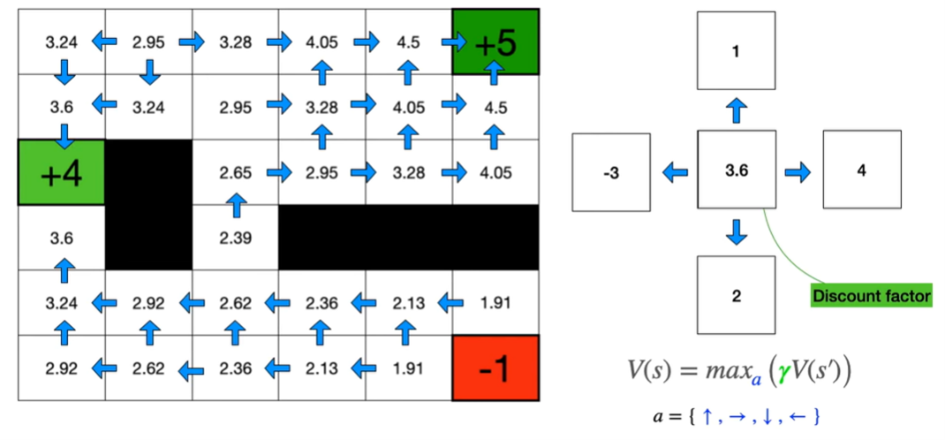
\includegraphics[width=0.8\linewidth,keepaspectratio]{rl39}
\end{center}

{\tiny (Ref: A friendly introduction to deep reinforcement learning, Q-networks and policy gradients)}

\end{frame}

%%%%%%%%%%%%%%%%%%%%%%%%%%%%%%%%%%%%%%%%%%%%%%%%%%%%%%%%%%%%%%%%%%%%%%%%%%%%%%%%%%
\begin{frame}[fragile]\frametitle{Example}

\begin{center}
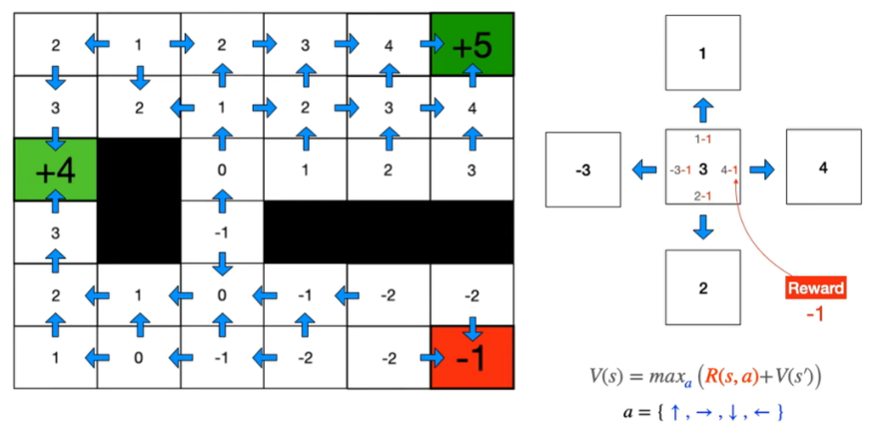
\includegraphics[width=0.8\linewidth,keepaspectratio]{rl38}
\end{center}

{\tiny (Ref: A friendly introduction to deep reinforcement learning, Q-networks and policy gradients)}

\end{frame}

%%%%%%%%%%%%%%%%%%%%%%%%%%%%%%%%%%%%%%%%%%%%%%%%%%%%%%%%%%%%%%%%%%%%%%%%%%%%%%%%%%
\begin{frame}[fragile]\frametitle{Example}

Bellman equation is combination of both

\begin{center}
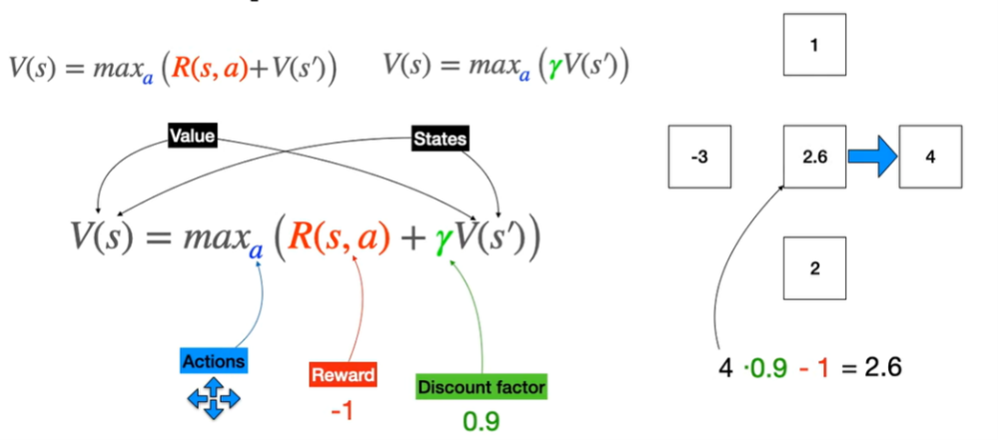
\includegraphics[width=0.8\linewidth,keepaspectratio]{rl40}
\end{center}

{\tiny (Ref: A friendly introduction to deep reinforcement learning, Q-networks and policy gradients)}

\end{frame}

%%%%%%%%%%%%%%%%%%%%%%%%%%%%%%%%%%%%%%%%%%%%%%%%%%%%%%%%%%%%%%%%%%%%%%%%%%%%%%%%%%
\begin{frame}[fragile]\frametitle{Example}

Start random, assign based on equation, keep updating. Iterate till settles. Policy is, ie with arrows

\begin{center}
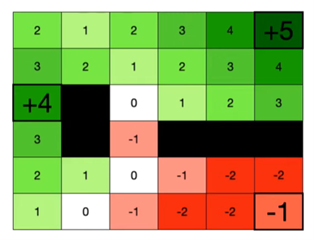
\includegraphics[width=0.35\linewidth,keepaspectratio]{rl41}
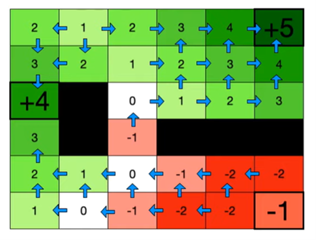
\includegraphics[width=0.35\linewidth,keepaspectratio]{rl42}

\end{center}

{\tiny (Ref: A friendly introduction to deep reinforcement learning, Q-networks and policy gradients)}

\end{frame}

%%%%%%%%%%%%%%%%%%%%%%%%%%%%%%%%%%%%%%%%%%%%%%%%%%%%%%%%%%%%%%%%%%%%%%%%%%%%%%%%%%
\begin{frame}[fragile]\frametitle{Example}

For many states, actions, iterating is very expensive. This is where neural networks come in. Two ways: Value network or Policy Network.
\begin{itemize}
\item Value network (Q networks): input is coordinates of the location; output is value.
\item Policy network: input is coordinates of the location; output is policy, i.e., probability of 4 actions.
\end{itemize}


{\tiny (Ref: A friendly introduction to deep reinforcement learning, Q-networks and policy gradients)}

\end{frame}

%%%%%%%%%%%%%%%%%%%%%%%%%%%%%%%%%%%%%%%%%%%%%%%%%%%%%%%%%%%%%%%%%%%%%%%%%%%%%%%%%%
\begin{frame}[fragile]\frametitle{Example}

Start with random values of neighbors. What should be value in the middle to solve bellman equation? That becomes label and then do back-propagation.

\begin{center}
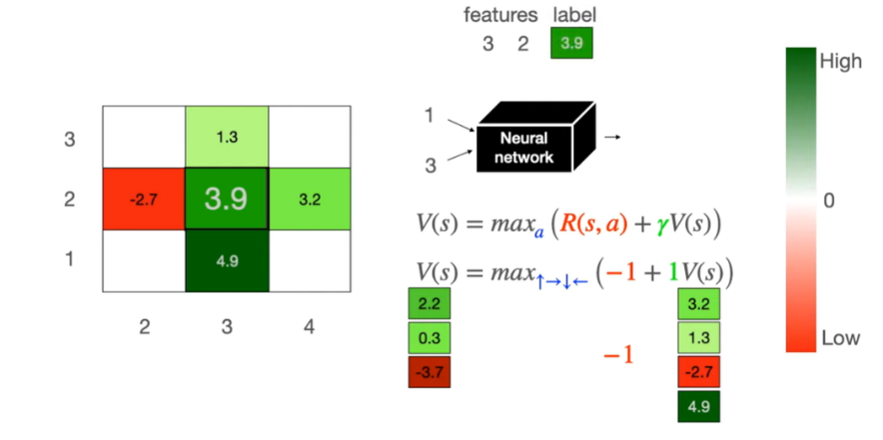
\includegraphics[width=0.8\linewidth,keepaspectratio]{rl43}
\end{center}

Once values are filled. We ask agents to take maximum value path.

{\tiny (Ref: A friendly introduction to deep reinforcement learning, Q-networks and policy gradients)}

\end{frame}

%%%%%%%%%%%%%%%%%%%%%%%%%%%%%%%%%%%%%%%%%%%%%%%%%%%%%%%%%%%%%%%%%%%%%%%%%%%%%%%%%%
\begin{frame}[fragile]\frametitle{Example}

For policy network, each location gives 4 direction probabilities. Then find path. Then from known value back trace the path by giving decreasing values. All the locations in the path become training rows.

\begin{center}
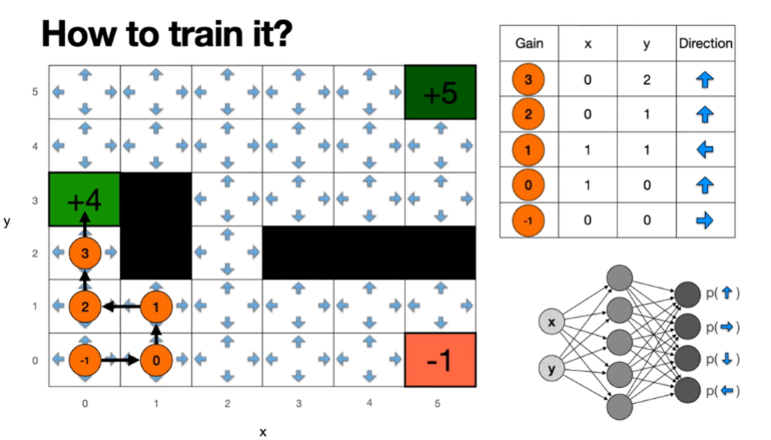
\includegraphics[width=0.8\linewidth,keepaspectratio]{rl44}
\end{center}


{\tiny (Ref: A friendly introduction to deep reinforcement learning, Q-networks and policy gradients)}

\end{frame}